\chapter{Implementation and Testing}

This chapter presents how the Jadwal system was implemented, detailing the technologies, services, and components that make up the deployed system. It also covers the security strategies, database adjustments, and testing practices used to ensure performance and reliability.

\section{Technologies and Tools Used}

Jadwal is built using a carefully selected stack of languages, technologies, and tools that enable fast iteration, strong security, ease of development, and deployment flexibility. Every choice made reflects our priority for speed, maintainability, and a high-quality user experience.

\subsection{Backend}

\begin{itemize}
    \item \textbf{Golang} – The main language used in the backend. It is a compiled language that generates native machine code (not bytecode), providing high performance and low overhead. Go also supports cross-compilation, meaning we can build binaries for different platforms (macOS, Linux, Windows) and architectures (x86, arm64) without requiring physical access to those systems. This was essential for our CI/CD and deployment process.
    \item \textbf{ConnectRPC} – The RPC framework we used to define our API. It is highly efficient and uses Protocol Buffers (protobuf) for serialization. This improves communication speed and ensures a consistent, type-safe interface between backend and frontend.
    \item \textbf{sqlc} – A Go-based SQL compiler. Unlike traditional ORMs that abstract SQL (and often add unnecessary complexity), sqlc lets us write raw SQL while still generating typed Go code. This gives us type safety and full SQL control — the best of both worlds.
    \item \textbf{migrate} – Used to handle schema migrations. Written in Go, it allows us to create up/down migration files and execute them at runtime. We also automated it to run at app startup, making database updates smoother during deployment.
    \item \textbf{RabbitMQ} – Our message broker used to decouple the WhatsApp message extraction service from the backend logic. It provides robust, asynchronous communication with delivery guarantees, retries, and scaling potential.
    \item \textbf{OpenAI-based LLM API} – Used in our event extraction pipeline to analyze and classify incoming WhatsApp messages. The abstraction allows easy model switching in the future without changing core logic.
    \item \textbf{HTTPJ} – A REST utility server that handles lightweight jobs like `.mobileconfig` file downloads. While not a central component, it simplifies small tasks that don’t need full RPC wiring.
    \item \textbf{Baikal} – An open-source CalDAV server written in PHP. It handles calendar data storage and sync and was reused in our system to provide a standards-based calendar integration layer.
\end{itemize}

\subsection{Frontend (iOS)}

\begin{itemize}
    \item \textbf{SwiftUI} – The framework used to build the iOS UI. It offers declarative, responsive UI development and is well-suited for small teams due to its simplicity.
    \item \textbf{EventKit} – Apple's official framework for accessing and managing calendar data on-device. It is used to read events, create prayer reminders, and add WhatsApp-parsed events.
    \item \textbf{Xcode} – Apple's IDE used to build, test, and debug the app. Also used for handling provisioning profiles and release builds.
    \item \textbf{JWT (JSON Web Token)} – Used for stateless authentication. Each user receives a signed token after login, which includes their identity (email/user\_id) and is verified using digital signatures to prevent tampering.
    \item \textbf{APNs (Apple Push Notification Service)} – Used to send push notifications for new events, conflicts, and reminders. We collect device IDs and securely store them to trigger these updates.
\end{itemize}

\subsection{WhatsApp Service (Wasapp)}

\begin{itemize}
    \item \textbf{TypeScript} – The main language for the Wasapp service.
    \item \textbf{bun.sh} – Used as our runtime for TypeScript — fast, modern, and integrates well with our stack.
    \item \textbf{Fastify} – A high-performance Node.js framework used to expose an API to the backend from the Wasapp service.
    \item \textbf{whatsapp-web.js} – JS client library that connects to WhatsApp Web, receives messages in real time, and emits events. This is the heart of our message extraction logic.
\end{itemize}

\subsection{Infrastructure, Deployment, and DevOps}

\begin{itemize}
    \item \textbf{Hetzner Cloud} - Cheap VPS provider in Europe with reliable service. We were able to run our project on a server with \textit{4 vCPU} and \textit{8gb ram} for \textit{€5.99/month}!
    \item \textbf{Docker} – Everything runs in containers: backend, Wasapp, CalDAV, etc. This enables consistent environments between dev and production.
    \item \textbf{Docker Compose} – Used to orchestrate services locally and during staging. Ensures that every developer gets the same setup out of the box. We used overlays, to override values between production and local environment along with `.env' files.
    \item \textbf{Traefik} – Our reverse proxy/load balancer/API gateway. It integrates with Docker, automatically issues SSL certs via Let's Encrypt, and handles SSL termination (internal services communicate over HTTP for performance).
    \item \textbf{GitHub} – Our version control system, CI/CD pipeline, and GitOps source of truth.
    \begin{itemize}
        \item \textbf{GitHub Actions} – CI workflows for building, testing, and pushing Docker images to GitHub Packages.
        \item \textbf{GitHub Packages} – Our Docker registry. Stores built images and lets us pull them easily on the server.
        \item \textbf{BlackSmith} – A third-party CI runner provider that gives us faster runners at lower cost. Speeds up builds and saves credits.
    \end{itemize}
    \item \textbf{Cloudflare} – Handles DNS, provides DDoS protection, serves as our CDN edge, and allows cheap domain registration. We also use it to force HTTPS and cache public assets.
    \item \textbf{Taskfile} – A Go-based task runner. We use it to alias common dev commands, test scripts, and deploy workflows into short commands.
\end{itemize}

\subsection{Database and Security}

\begin{itemize}
    \item \textbf{PostgreSQL} – Our main database. Used to store customers, calendar connections, event metadata, WhatsApp messages, device IDs, and more.
    \item \textbf{Beekeeper Studio} – A SQL GUI that lets us explore, debug, and visualize our PostgreSQL database. Used frequently during development.
    \item \textbf{Encryption at Rest (WhatsApp)} – We encrypt WhatsApp messages before storing them to protect user privacy in the case of a breach or access by other services.
    \item \textbf{Scratch Docker Images} – Our Go binaries are compiled statically and run inside Docker images built `FROM scratch`, meaning the containers are literally empty — no shell, no package manager, nothing for an attacker to exploit.
\end{itemize}

\subsection{Design, Documentation, and Diagrams}

\begin{itemize}
    \item \textbf{LaTeX} – Used to write this entire report. It handles figure references, bibliography, equation rendering, and allows us to store the report in version control for collaboration.
    \item \textbf{PlantUML} – Used to make sequence and class diagrams using plain text that can be rendered as SVG or PNG.
    \item \textbf{Mermaid} – Used for Gantt charts and simple flow diagrams, especially in markdown files and web-based previews.
    \item \textbf{Draw.io} – Used when text-based tools are too limited. We still track the `.drawio` files in GitHub for versioning.
    \item \textbf{UMLet} – Lightweight UML diagram tool used to make clean use case diagrams.
\end{itemize}

\subsection{Design and Productivity Tools}

\begin{itemize}
    \item \textbf{Figma} – Used to design our app logo, UI mockups, and presentation slides.
    \item \textbf{VS Code} – Our primary code editor. Supports extensions, Git integration, LaTeX building, and everything else we needed.
    \item \textbf{Linear} – Used for high-level project planning. Initially we tried micro-planning with it, but the project moved too quickly. We stuck to major task tracking and daily syncs.
    \item \textbf{Resend} – A transactional email service. We use it to send welcome emails, magic links, and other system emails. It has a generous free tier and works reliably.
    \item \textbf{PostHog} – A powerful analytics tool that tracks usage funnels, sessions, and user behavior. It enabled us to see session replays and understand user flows without asking users directly.
\end{itemize}

\section{System Architecture Realization}

The system architecture realization, compared to the architecture in \textbf{Figure~\ref{fig:architecture}}, was implemented using a modular, containerized structure. As shown in \textbf{Figure~\ref{fig:architecture-realization}}, all core components were packaged as separate services and deployed using Docker Compose on a single host. These include the backend service (Falak), the WhatsApp service (Wasapp), the CalDAV server (Baikal), a PostgreSQL database, and a Traefik proxy for HTTPS termination and service routing.

While the design envisioned a distributed system, the final implementation runs on a single host with isolated containers communicating over internal Docker networks. This setup preserves modularity and mirrors real-world deployment environments, while simplifying development and debugging. Each service is decoupled and can be scaled independently in future production-grade deployments.

The implemented architecture maintained full alignment with the original design, with minor practical adjustments such as unified logging using Grafana + Loki, simplified internal networking, and local queues (RabbitMQ) for event-driven flows. Overall, the implementation delivered on the designed goals of modularity, maintainability, and separation of concerns.

\begin{figure}[!h]
    \centering
    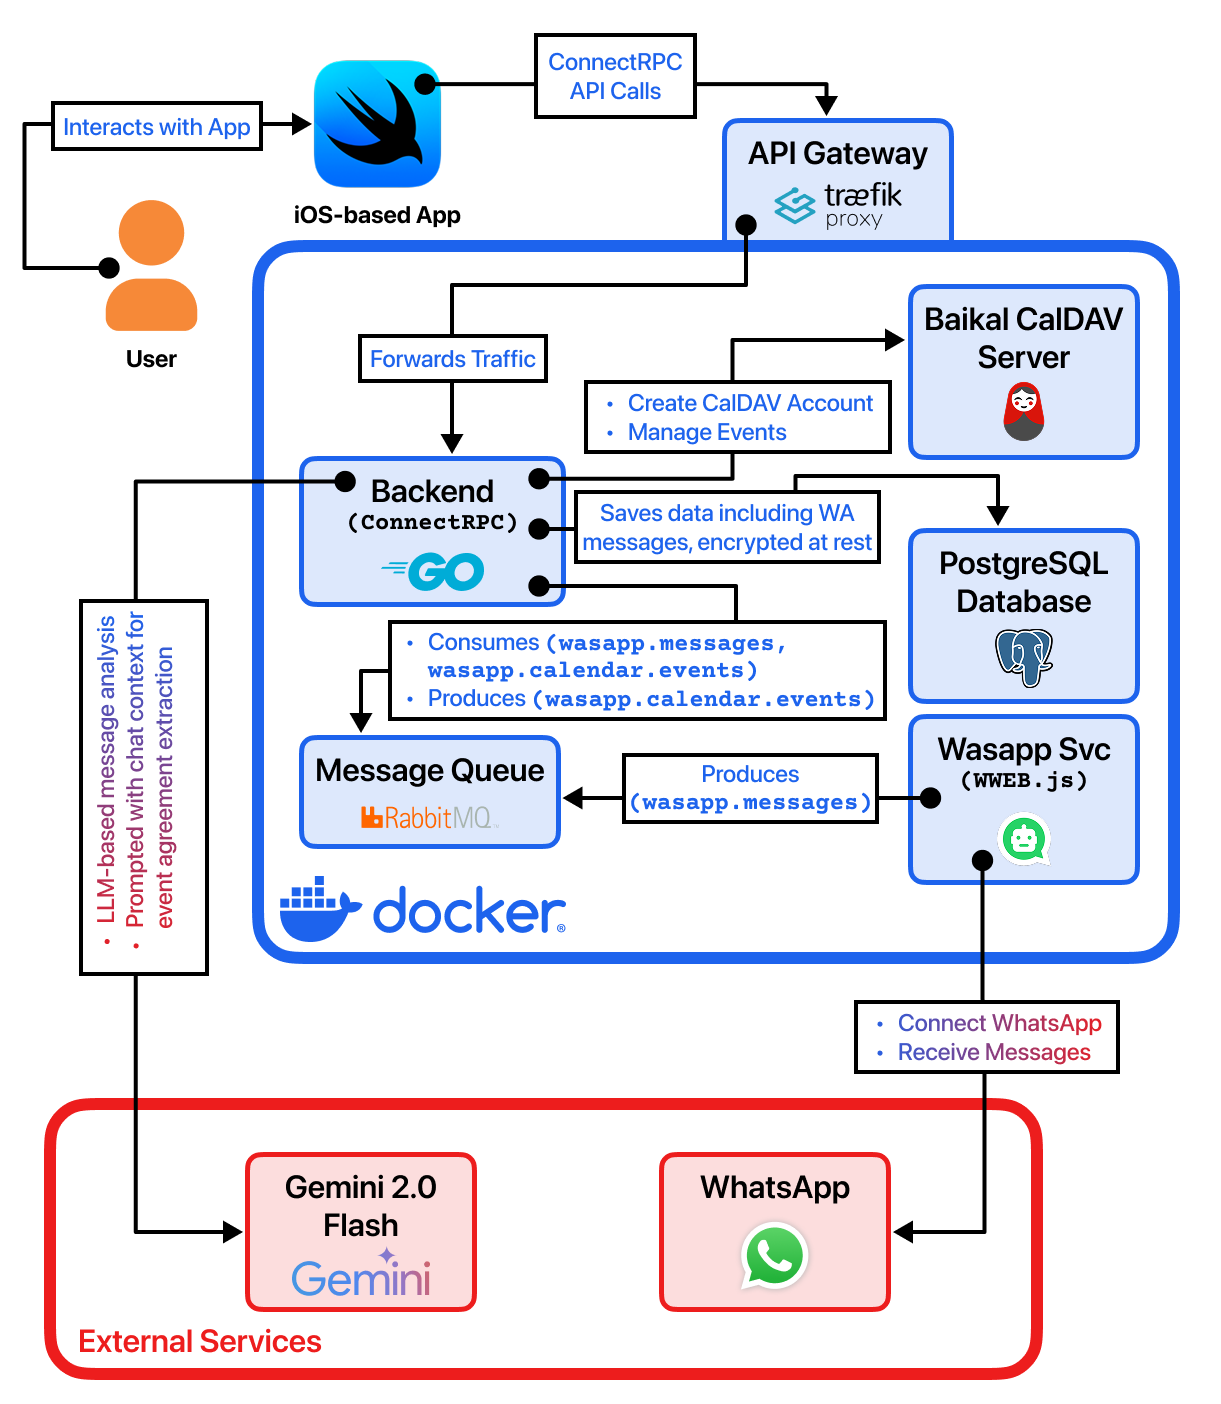
\includegraphics[width=0.8\textwidth]{images/system-architecture-realization.png}
    \caption{System Architecture Realization of Jadwal}
    \label{fig:architecture-realization}
\end{figure}

\section{Controlled Libraries}

In Jadwal, we intentionally selected controlled libraries and frameworks to ensure reliability, maintainability, and performance across the system. These libraries were carefully evaluated before integration to align with the project’s goals and security requirements. The following were key controlled libraries used:

\begin{itemize}
    \item \textbf{ConnectRPC} – For designing type-safe APIs between the backend and the mobile app.
    \item \textbf{sqlc} – For generating safe database access code from raw SQL queries.
    \item \textbf{whatsapp-web.js} – For handling WhatsApp web sessions and receiving messages programmatically.
    \item \textbf{Baikal} – As the controlled CalDAV server to manage calendars and events according to WebDAV standards.
    \item \textbf{RabbitMQ} – For handling asynchronous communication between services via message queues.
    \item \textbf{PostHog} – For session replay, funnel analysis, and usage tracking in a self-hosted, secure way.
\end{itemize}

The careful selection of these controlled libraries ensured that Jadwal maintained full control over its critical functionality while leveraging proven open-source technologies.


\section{Database Implementation}

The original database design, illustrated in Figure~\ref{fig:er-diagram} and Figure~\ref{fig:relational-schema}, was adapted during the actual system implementation. Initially, we planned to manage calendar storage directly within our own database schema. However, during development, we decided to integrate Baikal — an open-source, self-hosted CalDAV server — to handle calendar data following the CalDAV standard.

As a result, several tables from the original ERD were removed or replaced. The Falak backend continues to manage user accounts, authentication methods, WhatsApp message extraction, device IDs, and notification tracking, while Baikal independently handles all calendar-related storage.

The updated database design for the Falak backend, reflecting these changes, is shown in Figure~\ref{fig:updated-er-diagram} and Figure~\ref{fig:updated-relational-schema} below.

\begin{figure}[!h]
    \centering
    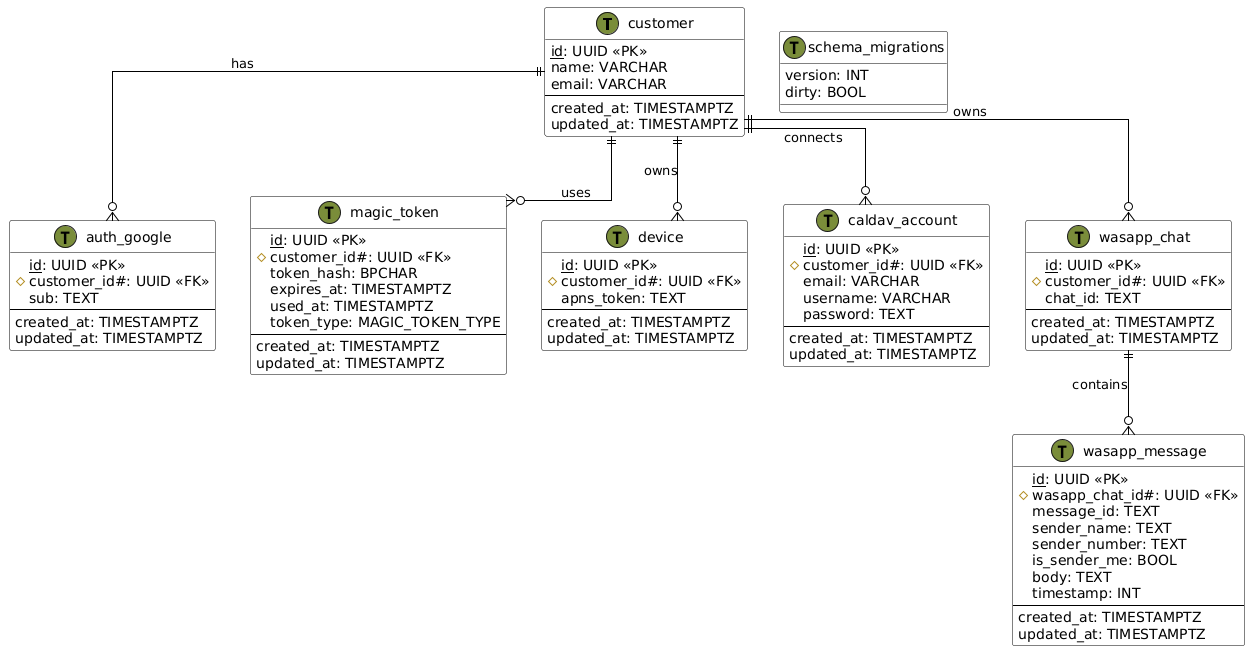
\includegraphics[width=0.9\textwidth]{images/docs/diagrams/er/new-database/Updated Falak ERD.png}
    \caption{Updated Entity-Relationship Diagram (Falak)}
    \label{fig:updated-er-diagram}
\end{figure}

% TODO: make this a relational one with draw.io, based on the one above :D
% \begin{figure}[!h]
%     \centering
%     \includegraphics[width=\textwidth]{images/updated-database-schema-relational.png}
%     \caption{Updated Relational Schema (Falak)}
%     \label{fig:updated-relational-schema}
% \end{figure}

\subsection{Baikal Database Schema}

To handle calendar event storage, we integrated Baikal directly without modifying its schema. Baikal follows WebDAV and CalDAV standards and manages calendars, events, user principals, and contact address books internally.

The key Baikal tables relevant to Jadwal's functionality are summarized below:

\begin{itemize}
    \item \textbf{calendars} — Stores metadata for user calendars.
    \item \textbf{calendarobjects} — Stores individual calendar events in iCalendar format.
    \item \textbf{calendarinstances} — Links calendars to user principals.
    \item \textbf{principals} — Represents authenticated users within Baikal.
\end{itemize}

Other tables related to address books, scheduling, and WebDAV-specific functionality (e.g., locks, subscriptions) were unused in our implementation. Baikal's database provided a mature and reliable backend for event storage without requiring us to reinvent a full calendar system.


\section{Implementation of Core Functionalities}

\subsection{Authentication} \label{subsec:authentication}

The authentication flow supports both magic links (email-based) and Google OAuth. Users receive a signed JWT upon authentication, which is used for subsequent requests.

We call it authentication since we don't differentiate between making an account and logging in — the user simply `continues' with a method, either Email with Magic Link or Google OAuth. If they already have an account, we just give them a token; if they don't, we create an account, send a welcome email, and then give them the tokens.

We generate access tokens (short-lived) and refresh tokens (long-lived), which are stored securely on the device. Magic tokens are hashed using SHA-256 before being stored in the database. For added security, we invalidate the refresh token upon logout, and all tokens are verified using digital signatures.

The login flow is fully stateless and scalable. We implemented it using ConnectRPC to ensure it works smoothly not just for iOS but also for future clients like a web app.

\subsection{Connect WhatsApp}

Connecting the user's WhatsApp account is an important feature. It allows Jadwal's system to securely read the user's messages (after encryption) to analyze them for events or meeting agreements using an LLM, more on that in Subsection~\ref{subsec:whatsapp-event-extraction}.

The process starts when the user clicks `Connect WhatsApp' in the app. They are asked to enter their mobile number, and once they submit, the Falak backend talks to the Wasapp service to create a new WhatsApp session.

The user is shown an 8-character code to enter inside the official WhatsApp app. We also deep-link the user into the correct screen in WhatsApp if possible. If not, the app gives clear instructions on how to manually reach it.

This method — using a code instead of QR scanning — makes the experience smoother on the same device. The app polls Falak to check connection status. If it fails, they can retry; if it succeeds, the user sees a success screen explaining that Jadwal is now securely monitoring messages.

On the server side, we launch a Chrome instance using whatsapp-web.js. Our Wasapp service abstracts this with an API that lets Falak create sessions, delete them, and check their status.

When connected, the Wasapp service produces the received messages into a RabbitMQ queue (wasapp.messages), ready for backend processing (see Subsection~\ref{subsec:whatsapp-event-extraction}).

\subsection{View Integrated Calendar}

When a user first opens Jadwal, they are asked for permission to access their on-device calendars. This allows us to show an integrated calendar view, month by month, without building a full CalDAV server and client — which would have been too ambitious for the time frame and hard due to limited online resources.

Instead, we used Baikal as a ready CalDAV server. We create accounts for users and let iOS handle syncing via its already battle-tested Calendar app integration (more about setup later in Subsection~\ref{subsec:connect-calendar}).

Users can view, add, and edit events directly inside the Jadwal app with a familiar native-like experience, ensuring ease of use.

\subsection{Prayer Time Scheduling} \label{subsec:schedule-prayer-times}

This feature is designed for our Muslim users — and since Alhamdulillah all project authors are Muslim and live in a Muslim country, it was something important for our community, which is often ignored by global apps.

The user clicks Schedule Prayer Times' inside the Settings tab. The app requests a generated .mobileconfig` profile based on the user's IP address to subscribe them automatically to a local prayer times calendar.

The user downloads the profile, installs it via Settings, and now their device automatically syncs prayer times into their calendar — visible both in the native Calendar app and inside Jadwal.

\subsection{WhatsApp Event Extraction} \label{subsec:whatsapp-event-extraction}

This is Jadwal's main innovation: automatic event extraction from WhatsApp messages using an LLM-powered classification pipeline.

Once a user connects their WhatsApp account, the Wasapp service (written in TypeScript with \texttt{whatsapp-web.js}) streams received messages to a RabbitMQ queue. A Golang consumer reads from this queue and sends the conversation context to an LLM — specifically, Google’s \textit{gemini-2.0-flash} model — which analyzes the thread to determine whether an event exists.

The prompt sent to the LLM includes the full message history wrapped in structured tags along with metadata such as current date and time. The prompt enforces strict constraints and expects a machine-readable JSON response with one of four statuses:

\begin{itemize}
    \item \texttt{NO\_EVENT}: No event detected.
    \item \texttt{HAS\_EVENT\_BUT\_NOT\_CONFIRMED}: An event was suggested but not confirmed.
    \item \texttt{HAS\_EVENT\_DENIED}: An event was suggested but rejected.
    \item \texttt{HAS\_EVENT\_AGREED}: An event was confirmed; additional fields like title, dates, and location are returned.
\end{itemize}

When an event is confirmed, it is published to the \texttt{wasapp.calendar.events} queue and added under the user’s special WhatsApp Events calendar. We also send an alert notification to inform the user, and a silent one to trigger conflict detection (see Section~\ref{subsec:conflict-resolution}).

The LLM integration is stateless and fully abstracted behind a Go service. During our testing, the system processed and extracted events faster than the original WhatsApp notifications arrived on the device.

For the full prompt template and formatting details, refer to Appendix~\ref{appendix:llm-prompt}.

\subsection{Conflict Resolution} \label{subsec:conflict-resolution}

Whenever a new event is added automatically by Jadwal, conflicts are checked.

Conflicts only matter for auto-added events (from WhatsApp) — because when users manually add events through the calendar view, they already notice conflicts directly.

Users can resolve conflicts through three actions:
\begin{itemize}
    \item \textbf{Keep New/Conflicting Event:} Acknowledge the conflict but keep it.
    \item \textbf{Move New/Conflicting Event:} Adjust the event timing.
    \item \textbf{Delete New/Conflicting Event:} Remove the new event.
\end{itemize}

The app presents a clean conflict resolution UI, showing side-by-side comparison of the old and new times for clarity. All UI, backend logic, and data handling for this feature were implemented successfully.

\textbf{Limitation:} The backend relies on a silent push notification to trigger conflict detection via the “Suggest Conflict Resolutions” use case. However, iOS's EventKit framework does let you \textbf{force fetch} the calendar's latest events when request, it just tries and sometimes is delayed by up to 5 minutes from our testing. This makes the feature unreliable in real-world usage and prevents us from reliably displaying the conflict resolution UI during testing.

\textbf{Future Work:} To overcome this, we need to implement a proprietary Apple protocol that is not public, but big companies use it. It allows the server to ``push'' updates to the client, in this case the iOS CalDAV implementation exposed via EventKit.

\subsection{Connect Calendar} \label{subsec:connect-calendar}

This feature makes it very easy for users to add the Jadwal CalDAV account to their phone.

Instead of manually typing the server URL, username, and password — risking mistakes — we let users click a button to download a \textit{.mobileconfig} file, install it, and have everything configured automatically.

The flow:

\begin{itemize}
    \item Click Easy Setup inside the app Settings.
    \item A short-lived (15-min) magic token is generated.
    \item The app opens a secure download of the mobile provisioning profile.
    \item The profile installs a CalDAV account automatically.
\end{itemize}

Magic tokens are hashed securely using SHA-256 and are one-time use only. The user barely notices all this complexity — for them, it’s just a smooth "click and go" experience.

\section{Our Journey in Getting to Baikal}

Originally, we thought about building our own CalDAV server — but quickly realized it was too ambitious given the time frame and how complex the CalDAV spec is.

We tried Radicale first (written in Python) but it lacked admin APIs we needed for user creation. Then we found Baikal, based on SabreDAV (a PHP WebDAV library) and used by serious projects like Nextcloud.

Baikal had everything we needed: CalDAV compatibility, admin dashboard, easy API, and Docker images ready. So we integrated it into our system, wrapped its API into our backend Falak service, and encrypted user credentials at rest.

When users connect their calendars via Easy Setup, they are actually connecting securely to Baikal through iOS’s native CalDAV system.

\section{System Security}

Security was a core consideration throughout Jadwal's development. The system is designed to protect user data both in transit and at rest, reduce attack surface, and isolate critical services from external access. The following measures were implemented to uphold a strong security posture:

\begin{itemize}
    \item \textbf{HTTPS Everywhere} – All traffic between mobile clients and servers is encrypted using TLS to ensure confidentiality and prevent tampering.
    \item \textbf{API Gateway with Traefik} – Traefik handles SSL termination, reverse proxying, and internal routing. It also supports automatic certificate renewal via Let's Encrypt.
    \item \textbf{Internal-Only Networking} – Core services like PostgreSQL, RabbitMQ, and monitoring tools are exposed only on the private Docker network, fully isolated from the internet.
    \item \textbf{Minimal Docker Images} – The Go backend is compiled into static binaries and run inside `FROM scratch` containers, resulting in extremely small, dependency-free images with no shell or package manager.
    \item \textbf{JWT-Based Stateless Authentication} – All requests are authenticated via signed JSON Web Tokens that include expiry and identity claims. Tokens are verified on every request via a middleware or interceptor.
    \item \textbf{Encrypted WhatsApp Messages} – WhatsApp messages are encrypted before being saved to the database to protect sensitive information in case of unauthorized access.
    \item \textbf{DNS \& DDoS Protection} – Cloudflare is used to manage DNS, enforce HTTPS, and provide protection against common web threats including DDoS and bot abuse.
\end{itemize}

\section{Testing Methodology}

Our testing methodology followed a black-box approach, emphasizing critical user flows such as email-based authentication, Google sign-in, and WhatsApp pairing. We relied on input space partitioning (ISP) for unit-level test design and used graph-based modeling for integration-level coverage.

PostHog was integrated to capture real user session flows and validate behavioral expectations. While full automation was not achieved, manual and programmatic testing throughout development helped us detect and resolve regressions early.

\section{Test Design}

\subsection*{Unit Test Design}

\subsubsection*{1. \texttt{InitiateEmail(String email)}}

\textbf{Description:} Validates the user’s email and sends a magic login link.  
\textbf{Test Technique:} Input Space Partitioning (ISP)

\begin{table}[h!]
\centering
\begin{tabular}{|c|c|c|c|}
\hline
\textbf{Block} & \textbf{A1} & \textbf{A2} & \textbf{A3} \\
\hline
\textbf{Email} & Valid format & Invalid format & Empty \\
\hline
\end{tabular}
\end{table}

\subsubsection*{2. \texttt{CompleteEmail(String token)}}

\textbf{Description:} Accepts a magic token from the link and authenticates the user.  
\textbf{Test Technique:} Input Space Partitioning (ISP)

\begin{table}[h!]
\centering
\begin{tabular}{|c|c|c|c|}
\hline
\textbf{Block} & \textbf{B1} & \textbf{B2} & \textbf{B3} \\
\hline
\textbf{Magic Token} & Valid & Expired or Invalid & Empty \\
\hline
\end{tabular}
\end{table}

\subsubsection*{3. \texttt{GoogleAuthentication(String idToken)}}

\textbf{Description:} Accepts a Google OAuth ID token and verifies it.  
\textbf{Test Technique:} Input Space Partitioning (ISP)

\begin{table}[h!]
\centering
\begin{tabular}{|c|c|c|c|c|}
\hline
\textbf{Block} & \textbf{C1} & \textbf{C2} & \textbf{C3} & \textbf{C4} \\
\hline
\textbf{idToken} & Valid & Expired & Malformed & Empty \\
\hline
\end{tabular}
\end{table}

\subsubsection*{4. \texttt{StartWhatsAppConnection(String phoneNumber)}}

\textbf{Description:} Starts the pairing process by accepting the user’s phone number.  
\textbf{Test Technique:} Input Space Partitioning (ISP)

\begin{table}[h!]
\centering
\begin{tabular}{|c|c|c|c|}
\hline
\textbf{Block} & \textbf{D1} & \textbf{D2} & \textbf{D3} \\
\hline
\textbf{Phone Number} & Valid format & Invalid format & Empty \\
\hline
\end{tabular}
\end{table}

\subsubsection*{5. \texttt{CheckWhatsAppConnectionStatus(String phoneNumber)}}

\textbf{Description:} Polls WhatsApp pairing status for a phone number.  
\textbf{Test Technique:} Input Space Partitioning (ISP)

\begin{table}[h!]
\centering
\begin{tabular}{|c|c|c|c|c|}
\hline
\textbf{Block} & \textbf{E1} & \textbf{E2} & \textbf{E3} & \textbf{E4} \\
\hline
\textbf{Connection Status} & Linked & Pending & Failed & Expired \\
\hline
\end{tabular}
\end{table}

\subsection*{Integration Test Design}

\subsubsection*{Email Authentication Flow}

The flow for email-based authentication is illustrated in Figure~\ref{fig:email-auth-flow}. The process begins when the user enters their email address into the app. The backend then triggers the \texttt{InitiateEmail} method, which sends a one-time magic link via email. When the user clicks the link, they are redirected back into the app, which captures the token embedded in the link. This token is then sent to the backend's \texttt{CompleteEmail} endpoint for validation. If valid, the backend issues access and refresh tokens, completing the login process.

\begin{figure}[h!]
    \centering
    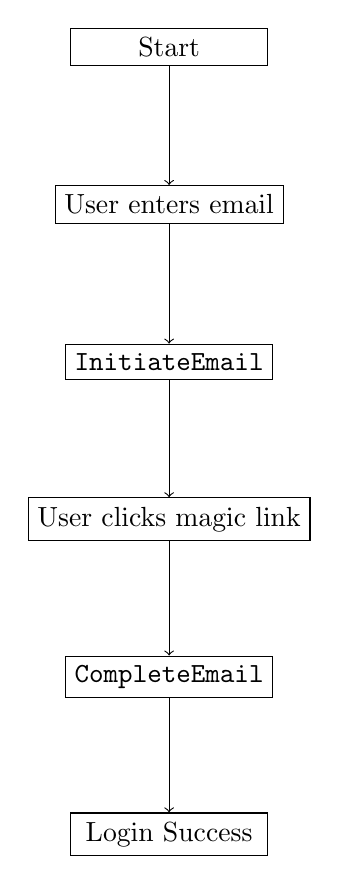
\begin{tikzpicture}[node distance=2cm, every node/.style={draw, align=center, minimum width=2.5cm}]
    \node (start) {Start};
    \node (enterEmail) [below of=start] {User enters email};
    \node (initiate) [below of=enterEmail] {\texttt{InitiateEmail}};
    \node (clickLink) [below of=initiate] {User clicks magic link};
    \node (complete) [below of=clickLink] {\texttt{CompleteEmail}};
    \node (success) [below of=complete] {Login Success};
    
    \draw[->] (start) -- (enterEmail);
    \draw[->] (enterEmail) -- (initiate);
    \draw[->] (initiate) -- (clickLink);
    \draw[->] (clickLink) -- (complete);
    \draw[->] (complete) -- (success);
    \end{tikzpicture}
    \caption{Email-Based Authentication Flow}
    \label{fig:email-auth-flow}
\end{figure}    

\subsubsection*{WhatsApp Connection Flow}

The WhatsApp connection flow is shown in Figure~\ref{fig:whatsapp-flow}. The user starts by entering their phone number, which is sent to the backend to initiate a pairing session using \texttt{StartWhatsAppConnection}. A unique pairing code is generated and displayed to the user. Meanwhile, the app begins polling the backend using \texttt{CheckStatus} to monitor the session state. The outcome of this polling could be one of three states: successful connection, still pending, or failure (e.g., user did not enter the code or session expired).

\begin{figure}[h!]
    \centering
    \begin{tikzpicture}[node distance=2cm, every node/.style={draw, align=center, minimum width=3cm}]
    \node (enterPhone) {Enter Phone Number};
    \node (start) [below of=enterPhone] {\texttt{StartWhatsAppConnection}};
    \node (showCode) [below of=start] {Show Pairing Code};
    \node (poll) [below of=showCode] {\texttt{CheckStatus} (poll)};
    \node (linked) [right of=poll, xshift=4cm] {Linked};
    \node (waiting) [below of=poll] {Still Waiting};
    \node (fail) [left of=poll, xshift=-4cm] {Failed};
    
    \draw[->] (enterPhone) -- (start);
    \draw[->] (start) -- (showCode);
    \draw[->] (showCode) -- (poll);
    \draw[->] (poll) -- (linked);
    \draw[->] (poll) -- (waiting);
    \draw[->] (poll) -- (fail);
    \end{tikzpicture}
    \caption{WhatsApp Pairing and Polling Flow}
    \label{fig:whatsapp-flow}
\end{figure}
    

\subsection*{OAuth 2.0 Flow for Google Authentication}

Figure~\ref{fig:oauth-flow} illustrates the OAuth 2.0 login flow used for Google authentication. The mobile app initiates the flow by redirecting the user to Google's consent screen. Upon user approval, Google returns an \texttt{idToken} to the app. The app then forwards this token to the backend, which verifies it using Google's public keys and extracts the authenticated user's identity. This flow ensures secure, federated login without requiring the app to handle passwords directly.

\begin{figure}[h!]
    \centering
    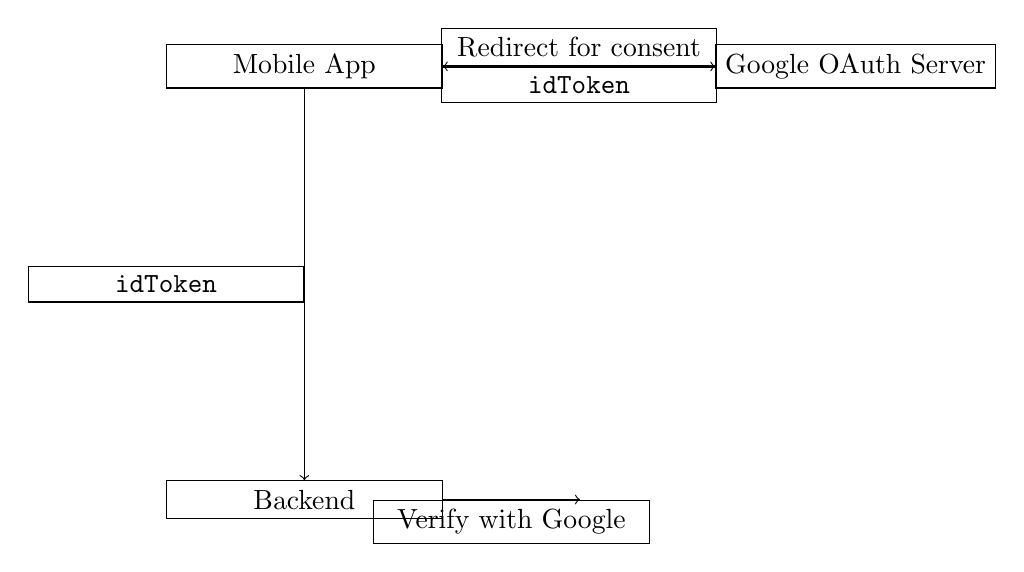
\begin{tikzpicture}[node distance=2cm, every node/.style={draw, align=center, minimum width=3.5cm}]
    \node (app) {Mobile App};
    \node (google) [right of=app, xshift=5cm] {Google OAuth Server};
    \node (backend) [below of=app, yshift=-3.5cm] {Backend};
    
    \draw[->] (app) -- node[above] {Redirect for consent} (google);
    \draw[->] (google) -- node[below] {\texttt{idToken}} (app);
    \draw[->] (app) -- node[left] {\texttt{idToken}} (backend);
    \draw[->] (backend) -- node[below] {Verify with Google} ++(3.5,0);
    \end{tikzpicture}
    \caption{Google OAuth 2.0 Flow with idToken Exchange}
    \label{fig:oauth-flow}
\end{figure}
    

\textbf{Why it matters:} The \texttt{idToken} is a signed JWT. We test it for validity, expiration, and structural integrity.

\subsection*{Integration Test Execution}

Each integration flow was tested end-to-end using a simulated user input and backend inspection.

\begin{itemize}
    \item \textbf{Email Authentication:} We verified that submitting an email via the app triggered a magic link via Resend, and that clicking the link opened the app and authenticated the user using the correct token. Failure cases were also tested using expired or tampered tokens.
    \item \textbf{WhatsApp Pairing:} After submitting a phone number, we confirmed that a pairing code was generated and exposed via API. We verified that polling detected the linked session and updated the UI accordingly. Error cases were simulated by expiring codes or intentionally triggering session errors.
    \item \textbf{Google OAuth:} The flow was tested using real Google test accounts. We confirmed that the app received a valid `idToken` and that the backend verified the token using Google's public keys. Failure cases included expired tokens, malformed tokens, and empty inputs.
\end{itemize}

In each flow, PostHog was used to observe real-time user actions, allowing us to validate the actual experience and detect any discrepancies between backend and frontend states.

For full test case executions and their actual outcomes, please refer to Appendix~\ref{appendix:test-execution}.

\section{Comparison to Original Specification}

During implementation, we made several changes to the original design while keeping the core goals of Jadwal intact. Some functional flows, such as calendar event management, were re-implemented using Baikal instead of a custom schema. Others, like WhatsApp event extraction and prayer time scheduling, were refined to better match technical feasibility and real user needs. While the internal structure of the system evolved significantly, especially in database design and service architecture, all critical functionalities promised in the original specification — authentication, event integration, scheduling, and notifications — were delivered. These changes were necessary to produce a system that is secure, maintainable, and production-ready.

\section{Runtime Evaluation}

Jadwal was built with speed, efficiency, and low-latency user experience in mind. The backend, implemented in Go, is compiled into a single native binary, resulting in fast startup and low memory usage. Our API calls typically respond in under 1 second under normal conditions. Calendar events are fetched and parsed quickly, and WhatsApp message processing is handled asynchronously via RabbitMQ to avoid blocking operations. The use of stateless authentication (JWT) and local caching ensures smooth performance on the mobile app, even in poor network conditions. Overall, the system met or exceeded our original performance expectations.
